%&tex
\chapter{Introduction}
\label{cha:introduction}

% dramatic entry
Throughout history human aggression has demonstrated to what extend it can cause distruction and harm.
The nature and cause of such behavior has always been of interest to social and biological focused researchers and much scientific effort has been spend to investigate the various different facets of this complex behavior.
The complexty of this behavior is reflected in the importants it takes part within our societies in terms of art, music, theater and above all history.
Indeed, history books seem to be mostly about wars and reports of crime are represented to a significant part in our contemporary newspapers.
Thus it is not surprising that the origin and cause of such behavior has resulted in much controversy in the past.
Social scientists have argued in the past for exclusivly social causes of aggressive behaviors, most biological based researchers have argued for genetic causes.
This nature versus nurture debate is, however, outdated and today's scientific view acknowledghes both social and biological mechanisms of human aggression.

Here I will soly focus on potential biological mechanisms of human aggression.
Specifically I will investigate the genetic causes of human aggressive behavior via a variety of different statistical methods.
This includes a study on 28,000 twin pairs and a genome wide analysis of over 150,000 unrelated individuals.
Further I will discuss a newly developed statistical method to identify genes of interest associated with human aggression.
At last I will explore the effect the parental genetic background has on the behavior of their off-spring via the enviornment.
However, I will first define, explore evolutionary theories, and outline the biological mechanisms of aggressive behavior discussed in previous research. 

\section{Definition of Aggression}
\label{sec:overview_of_reseach_in_aggression}

One can define human aggression as a behavior intended to cause physical or emotional harm to others~\cite{Anderson2002}.
However, this definition is rather incomplete.
It is important to consider the unwilling participation of the victim as well.
Hence behaviors in which the target does not intend to avoid the aggressive behavior, such as in sexual masochism~\cite{Berkowitz1993,Baumeister1989,Baron2007,Geen2001} should not be considered an aggressive act.
Thus the motivation of the victim to avoid such harm plays an important role in the definition of aggressive behavior.  
Therefore I will use the following working definition:
\begin{mydef}[Aggression]\label{def:aggression}
	`Aggression is the delivery of an aversive stimulus form one person to another, with itent to harm and with an expectations of causing such harm, when the other person is motivated to escape or avoid the stimulus'~\cite{Geen2001}
\end{mydef}

While aggression is most commonly associated with physical harm, definition~\ref{def:aggression} also includes a more broader spectrum.
Like spreading gossips, damaging a victims property either due to emotional anger or as a planned action to gain an advantage to a higher goal.
The large spectrum of aggression makes it necessary to specify some more broader dimension of this behavior.

\subsection{Forms of aggression}
\label{sub:forms_of_aggression}

One can futher seperate aggressive behavior into \textit{affective aggression} and \textit{instrumental aggresssion}.
While \textit{affective aggression} is characerised as emotional, impulsive, thoughtless and unplanned behavior, \textit{instrumental aggression} is defined as a planed and proactive behavior to obtain a certain higher goal~\cite{Berkowitz1993,Geen2001}.
The distinction between certain types of aggression has been extended by a number of similar concepts, such as \textit{reactive/proactive} and \textit{offensive/defensive} aggression.
While these terms have slightly different meaning, depending on situtation and field of research, the general concept remains similar~\cite{Geen2001, Blanchard2005b}.
In psychology, for example, the term \textit{affective aggression} and \textit{instrumental aggresssion} has been establised, but more recently authors have used the terms \textit{reactive} and \textit{proactive} aggression~\cite{Geen2001}.
Thus aggressive action in response to a provocation, such as self-defence and in anger, is \textit{reactive aggression} while planned, un-provoced aggression is called \textit{provocative}.

However, despite the differences in terminology it is important to emphasise the strong negative emotional state of \textit{affective/reactive} aggression.
This state, often descibed as \textit{anger}, launches and guids affective aggression  and is often caused by some form of provocation\cite{Geen2001}.
Nevertheless, \citet{Frijda1994} suggested that \textit{affective/reactive aggression} is not necessary impulsive.
In some situations a delayed response between provocation and aggressive response is observed. 
In particular long term grudges, or \textit{hatreds} are preoccupations which go beyond the initial provocation but remain deeply emotional.
Thus I will use the term \textit{impulsive aggression} to refer to impulsive, emotional guided aggressive behavior.

In contrast \textit{Instrumental/proactive aggression} is characerised by the absence of an emotional strong cause to cause harm.
For example, the use of gossip and bad-mouthing of a colleague in order to obtain higher chances of receiving a promotion is done in a planned manner with the aim of a higher goal (receiving the promotion).
However, it is often difficult to distiguish actions into affective and instrumental aggression since both forms are not mutually exclusive.
\citet{Geen2001} gave the example of a mother who uses corporal punishment to modify her child's behavior, while still reacting in anger when observing the undesired child's behavior.
Hence mixing a planned aggressive act with a higher goal with an aggective state.

Both forms of aggression, affective and instrumental, can be either physical or verbal.
While physical aggression in humans is homologous to other animals, verbal aggression, also called indirect, relational and social aggression, is relativly distinct to humans~\cite{Archer2005}.
These verbal behaviors cause harm to others by gossiping, spreading rumors, or excluding other from social groups.
While the terms \textit{indirect}, \textit{relational}, and \textit{social} aggression have been differently conceptulized in the past~\cite{Archer2001}, they are expressed in common behaviors and can be contrasted to physical aggression.
Hence the terms are more similar than distinct and I will therefore proceed to call all them \textit{indirect} aggression in order to distiguish it more from the physical, more direct aggressive behavior\cite{Archer2005}.

Research in animals have often used a slightly different terminology.
Investigations often have distiguished between \textit{offensive} and \textit{deffensive} aggression~\cite{Blanchard2005b}.
Similar to \textit{affective} aggression \textit{offensive} attacks arise from a response to a threat to the animals resources, thus are the response to a certain provocation.
These resources could be sexual partners, food, social status, or in the case of humans, also money.
On the other hand \textit{deffensive} aggression is the result to a direct threat to the subject life, a concept closer related to \textit{instrumental} aggression.
While this distingen might hold in mice and rats, the seperation between \textit{offensive} and \textit{deffensive} aggression is more blured in primates, including humans.
For example, humans are known to hunt lions and other predators.
In contrast to non-predators, these animals are, for the most part, not eaten which would suggest a form of deffensive aggressive behavior.
However, within most human cultures killing a large predator is seen to enlarge ones social status by showing strenght and courage towards the others.
A behavior which could be described as an \textit{offensive} action.
Thus the distinction between \textit{offensive} and \textit{deffensive} aggression is blured.
This blured distinction reflects the above described example of the punishing mother by \citet{Geen2001}.
However, \citet{Blanchard2005b} suggest, while the distinction between \textit{offensice/affective} a and \textit{defensive/instrumental} might be blured in humans, the distiction holds in general.
The authors suggest that rather insufficient analysis and not a disconnetion between animal and human behavior are responsible for the blured distiction within humans.
However, \citet{Blanchard2005b} provide little evidence for their claims and one can argue that the complexity of human society makes a comparison between sub-categories of aggressive behavior across species especially difficult. 
Nevertheless, animal studies have provided valuable insight into aggressive behavior and I will outline a number of experimental findings in animal studies in later sections.

To conclude, one can distiguish between \textit{affective} and \textit{instrumental} forms of human aggression which can be expressed either \textit{direct} or \textit{indirect}.
Research in non-humans have often distiguished between \textit{offensive} and \textit{deffensive} forms of aggression.
A distiction which is more blured in humans.
I will next consinder evolutionary theories considering aggression in humans and animals alike.
I will show that aggressive behavior has a strong evolutionary background and that genes which regulate such behavior are under stabilizing selection.

\section{Evolutionary Theories}
\label{sec:evolutionary_theories}

Historically, research of aggression has been devided into nurture versus nature~\cite{Archer2009}. 
Proponents of the nurture side have argued that aggressive behavior is caused by enviormental influences, while supports of the nature side of the discussion supported the idea that only differences in the genetic architecture are able to explain individual differences in aggressive behavior.
Today's view is less polarized and acknowledghes that both, nature and nurture play a crucial part in aggression.
While not disregarding the enviormental aspect of aggression I will mostly focus on the genetic and biological mechanisms of aggressive behavior.
In the following section I will outline evolutionary concepts helpful in explaining individual differences of aggression. 
\vfill
Evidence for a long history of human aggression can be found in  paleontological findings of broken bones, rips and smashed skulls, unexplainable without the consideration of weaponary force, and occasional findings of weapon fragments in skeletal rib cages suggest that violence and aggression has been part of the human evolutionary history. 
\citet{Buss1997}, one of the founder of evolutionary psychology, suggested that all psychological mechanisms and behavior, including aggression, originate in the evolutionary priciple of selection.  
These mechanisms are aimed to solve specific adaptive problems.
Hence some variants of those behaviors and psycholigcal mechanisms might solve certain problems better than others, improving overall fitness.
This results in the preservation, replication and spreading of theses variants throught a population~\cite{Buss1997}.
Hence, from a evolutionary perspective, every human behavior can be seen as a solution to a specific adaptive problem.
Therefore aggression is, from an evolutionary view, an adaptive problem solving mechanism.

\citet{Buss1997} suggested \textit{seven} adaptive problems to which aggressive behavior might be an evolutionary solution.
For example \textit{Co-Opt the Resources of Others}, which can be defined as the use of physical or psycholigcal force to obtain resources hold by another indivudual or group, can give the aggressors significant advantages in terms of survival and reproduction.
These resources could mean food, water, land or secual partners.
An example of this can be seen in aggressive behavior of children.
\citet{Campbell1995} noted that aggression among toddlers is often about resouces, such as toys, suggesting that this behavioral adaptations is an deeply rooted evelutionary strategy.

As discussed above, aggression can also be useful in \textit{defending against an attack}.
Since attacking aggressors are a serious threat to valuable resources.
Aggression can be an effective strategy in defending against indivuduals or groups.
Further, it can be also an adaptive strategy to foster a reputation that would deter potential aggressors~\cite{Buss1997}.
Thus avoiding the potential cost of a physical conflict while defending one's resources.

Another evolutionary benefit of aggression can be found in the social hierarchies in groups.
For example, men who win fights and defeat opponents gain power and status in many societies~\cite{Hill1996}.
The gain in social status can be beneficial in accessing resources and mates~\cite{Archer2009}.
Indeed, hirarical order in social groups is often established by means of aggressive behavior which enables high ranked individuals prioriy access to food and paterns~\cite{Lindenfors2011}. 
However, aggression can also result in an decline in status.
\citet{Buss1997} suggested for example that a physical conflict between two professors in a facutly meeting would result in an decline in repuatation.
Thus display of aggression is not acceptable in all social situations.

In the context of reproduction one should consider aggression towards the same-sex seperate of male-female aggression.
Aggression towards same-sex individuals is sometimes aimed to reduce their social status and therefore make them less attractive to the other sex~\cite{Buss1990}.
Hence inflicting damage on a rival directly translates to an incresed benefit to the aggresssor.
In addition to aggression towards same-sex individuals, aggression is also prevelant towards the oposite sex.
For example, aggression can be used to deter a long-term mate from infidelity~\cite{Daly1982}.
However, also here aggression can have negative consequences in form of retahilation.
For example, a husband might be reluctant to use aggression towards his wive when she is living close to a number of brothers and a powerful father.
Indeed, a study in Madrid, Spain found that women who had a higher density of genetic kin in and around Madrid were less likely to be victim of domestic violence~\cite{Figueredo1995}.
Hence aggression only brings an evolutionary advantage when the benefits outweight the potential costs.

Same-sex and male-female aggression is not equally balanced among the two sexes and nearly all mammals display sex differences in the expression of aggression.
Qualitative, the type of aggression, as well as quantitative.
In general males are more likely to exhibit physical aggression than female.
These sex differences have been discussed in the context of sexual selection theory (SST)~\cite{Archer2004,Anderson2002}. 
Sexual selection is concerned how a member of one sex choses another individual from the other sex, as well as the competion between members of the sex over access to the other~\cite{Darwin1859}.
In most mammals the more competitive sex is the male~\cite{Archer2009}. 
\citet{Trivers1972} suggested that these sex differences can be explained by the commonly observed reduced parental investment by males.
Parental investment is the amount of resources a parent investes into his or her off spring to increase its survivial and reproduction~\cite{Archer2009}.
The theory was first suggested by \citet{0198504403} and proposes that a male can minimize his parental investment in favor in producing a higher amount of offspring.
In contrast, many female mammals have an large obligatory patrental investment, such as gestation and delivery.
Thus female partner selection is more careful compared to male.
Hence the female selection of good reproductive fitness is directly linked to offset the lack of male paternal investment.
Since aggression is, as described above, often associated with an increased access to sexual partners one can conclude that this behavior is under sexual selection.

Despite these advatages, increased levels of aggressive behavior can also be harmful to the individual.
Expressing aggression towards another individual sheers energy away from other acitivies, such as hunting and foraging, and also carries a high risk of injury and death~\cite{Packer1995}.  
This increased cost is also reflected in the conflict resolving method applied across many animals and human.
For example, two competing male red deer may begin their confrontation by roaring repeatedly.
If this does not resolve the conflict both will walk side-by-side while attempting to make themself look as large as possible.
Only the last stage involes a physical confrontation, potentially causing sever injuries~\cite{Clutton-Brock1979a}.
These behaviors, aimed to resolve conflicts without the use of raw force, demonstrates the large costs of physical aggresssion.
However, it does also show that animals and humans alike are able to avoid those costs by threating the use of physical force.
\citet{Maxson2005} suggested that if the fighting ability of the resource holding power (\acrshort{rhp}) as well the resource value (\acrshort{rv}) are the same for both contestant, conflicts will usually escalate.

Despinte the advantages of using aggression to gain a higher social status there are considerable negative consequences.
In a study~\cite{Packer1995} on 138 female baboons in the Gombe National Park in Tanzania high-ranking females showed lower inter-birth intercals as well as higher offspring survival rates.
Thus one would expect higher life-time reproductive success in baboons with overall higher social rank acorss their life-time.
However, the authors were not able to associate reproductive success with mean life-time rank.
\citet{Packer1995} suggested that this inconsitency can be explained by considering that higher ranked females are also more likely to suffer a  miscarriages.
These stress-related failure in reproduction can be seen as a counter-force to a potential arms-race among female baboons.
Hence the induced aggression by competing for higher social status carries the cost of significant risk of misscarigas.

Therefore, the increase in fitness due to aggressive behavior, either as a direct gain in resources or higher social status, is balanced by large risks such as injuries, death, reduced reproduction and others.
This would indicate that aggression is under stabilizing selection (see figure~\ref{fig:stab}).

\begin{figure}[hp]
	\centering
	\scalebox{0.6}{\documentclass{minimal}
\usepackage{tikz}
\usetikzlibrary{positioning}
\begin{document}
\tikzstyle{box} = [rectangle, rounded corners, minimum width=3cm, minimum height=1cm,text centered, draw=black]
\begin{tikzpicture}
	\draw[line width=6, gray] (-7,0)-- (0,0) --(7,0);
	\draw[gray, fill=gray] (-1,-2)-- (0,0) --(1,-2) --(-1,-2);

	%Cost
	\node (injury) [box, fill=red!80] at (-5,0.6)  {Reproductive Cost};
	\node (grooming) [box, fill=red!70, above of=injury] {Foraging};
	\node (repo) [box, fill=red!60, above of=grooming] {Parental care};
	\node (foraging) [box, fill=red!50, above of=repo] {Grooming};
	\node (parCare) [box, fill=red!40, above of=foraging] {Injury risk};

	%Benefit
	\node (mat) [box, fill=blue!80] at (5,0.6)  {Mating priority};
	\node (res) [box, fill=blue!70, above of=mat] {Resource access};
	\node (def) [box, fill=blue!60, above of=res] {Predator defense};
	\node (surv) [box, fill=blue!50, above of=def] {Survival};
	\node (dom) [box, fill=blue!40, above of=surv] {Social Dominance};
\end{tikzpicture}
\end{document}
}
  \caption{Stabilizing selection of aggressive behavior (as in \citet{Anholt2012}). The benefit of aggressive behavior is countered by its cost. Thus maintaining a stable level of aggressive behavior within the population}
	\label{fig:stab}
\end{figure}

The above outlined cross-species and evolutionary history of aggressive behavior suggests thats inherited biological factors play a key role.
I have shown that aggression, while having large benefits for the aggressor, also caries significant drawbacks.
Hence aggressive beavior is under stabilizing selection.

In the following secton I will outline specific genetic aspects of aggression.
Due to the widespread use of aggressive behavior and the limits of genetic research in humans, genetic studies have mostly focused on nonhuman animals.
Further I will describe potential nerological mechanisms involved in aggression among mamals, as well as the role of hormones.
At last I will focus on studies on human, both in twins and adoption studies as well as genome wide association studies.


\section{Biological Mechanisms}
\label{sec:biological_mechanisms}

Most findings in regards to the genetics of aggressive behavior comes from animal studies and only few have come from studies on humans.
Hence previous research has made use of comparative genetics to gain insight into the gentics mechansims of human aggression.
Comparative genetics is the use and analysis of genomic information across species to identify and relate genes with phenotypes~\cite{Maxson2003}.
The comaprison across species to identify genes which are related to aggresssion has a number of advantages.
As outlined in section~\ref{sec:evolutionary_theories}, aggressive behavior is present in number of species which indicates that this particular bahvior is, form an evolutionary view, relativly old.
Thus a cross species perspectives enables to examine overlapping genes which might affect this particular behavior.
This not only allows to identify genes involved in aggression across species but also enables to consider neural mechanisms and gene-enviornment interactions similar in humans and non-humans alike.

Nevertheless, a number of different studies have investigated aggression in humans despite the described chalenges.
\citet{Maxson2005} proposed three general approaches to investigate the genetic architecture of aggressive behavior.
(1) One can identify genes by mapping their sequence to different forms of aggression (see my own study in chapter ???).
(2) Another approach is to alter the genetic code of experimental organisms, such as rats and mice, to test for the effects of different genes on aggression.
(3) Last, one can measure the rate of gene expression within the brain in association with an aggressive phenotype.
Only in recent years option (1) and (3) was made possible due to massive progress in the sequencing of human and animal genoms.
Option (2) has the highest scientific vadility due to the use of randomized control trials, a method only available in nonhuman animals due to ethical considerations.
However, one can also add a fourth category.
One can also investige DNA methylation in order to investigate the epigenetic mechanisms of aggressive behavior.
DNA methylation is used as a biological control mechanisms by the organism to control gene expression.
While studies on DNA methylation in human aggression have been only recently been conducted~\cite{VanDongen2015a} this new field of study is potentially promssing in investigating the genetic mechanisms of aggression.
Further, another method can be applied to investigate the genetic mechanisms of aggressive behavior.
However, association studies in humans face a number of chalenges.
The quantification of aggressive behavior via questionaire difficult due to the multidimentionality of the phenotype.
Further analysis of the whole genome does requrie considerable sample size.
These challgenes makes it very difficult to find new genetic risk factor for aggression.
Nevertheless, a number of studies have focused on only a handful of genes which were previously discovered in animal studies.


\subsection{Genetic Associations in Humans}
\label{sub:genetic_associations_in_humans}
While~\citet{Maxson2005} only described molecular methods on can also make use of twins.
Twin studies make use of the genetic similarity (or dissimilartiy) of dizygotic and monozygotic twins.
Since diszygotic twins, and siblings for that matter, share 50\% of their gentic markup with their brother or sister, monozygotic twins share 100\%.
This enables to estimate the genetic contribution of aggressive behavior in humans.
These studies have been a popular method to invesatigate the genetic contribution of a variety of different phenotypes and I will outline a detailed description of this particular method in section~\ref{chap:longHera}.
Most twin studies estimate the genetic contribution to aggressive behavior between 50\% and 80\%~\cite{Porsch2016}.
While these estiamtes give a broad understanding about the importance of genetic factors contribution on aggression twin studies are unable to inform about specific genes or genetic marker.

Genetic associations studies in humans, on the other hand, commonly face difficulties of obtaining large enogh sample sizes and therefore lack statisticial power.
Thus previous studies, as mentioned above, focused on only a handful selected genes to investigate the genetic architecture of human aggression.
However, single gene association studies often fail to replicte and are as well often uderpowered.
For example, alzheimer patiens which are homozygous for the \textit{apolipoprotein E e4} allele have been reported to be more at risk of expressing aggressive behavior~\cite{Craig2004a,VanDerFlier2006}.
However, these finding could not be replicated in a study with larger sample size~\cite{Hollingworth2006}.
Similar, studies on catechol-O-methyl transferase gene (COMT) in schizophrenia have associated a single polymorphism with aggression~\cite{Hirata2013,Calati2011} but the sample size of these studies are limited.
Thus one should view these results with caution.

Nevertheless, one well known genetic characteristic of aggressive behavior was discovered when analysing a rather large Dutch family~\cite{Brunner1993}.
In particular, male members of this family were knonw for their aggressive behavior, including arson, attempted rape and other forms of aggression.
Genomic analysis revlealed that individuals had a deficient monoamine oxidase due to a point mutation in the \textit{MAOA} gene.
A result which has been replicated multiple times in humans~\cite{Huang2004,Manuck2000} as well in mice~\cite{Cases1995b} and monkeys~\cite{Newman2005}.

The identification of \textit{MAOA} represents the first gene directly associated with aggressive behavior.
Further it put other neurotransmitter into focus, including serotonin~\cite{Murphy2008}, dopamine, norepinephrine, and GABA~\cite{Marino2005,Miczek2002}.
For example, \citet{Hohmann2009} indentified an association between a variable number tandem repeat (VNTR) and externalizing behavior in the dopamine D4 receptor (\textit{DRD4}) gene.
Interestingly, subjects which also had a mutation in the serotonin transporter \textit{SLC6A4}, specifically in the serotonin-transporter-linked polymorphic region (\textit{5-HTTLPR}), showed high levels of aggressive behavior.
This behavior was not present if only one of the two mutations were presents.
Hence this is a rare display of a gene-by-gene interaction, also called epistasis~\cite{Anholt2012}.

To conclude, genetic analysis in humans has shown multiple different potential genes implicated in human aggression.
Most prominently \textit{MAOA} as well as \textit{DRD4} in combination with \textit{SLC6A4}.
However, studies in humans have so far only focused on a few set of candidate genes due to the high costs associated with an analysis of the whole genome.

\subsection{Genetic Associations in nonhuman animals}
\label{sub:genetic_associations_in_animals}

Genetic analysis in animals have a number of advantages.
First, one is able to make direct manipulation of the genome in question and second, one is able to quantify aggressive behavior more easaly.
For example, aggression in mice can be measured by counting the number of attacks the animal perfoms when placed in a situation which involves social confrontaion with another mouse.

A number of studies have investigated the effect of different neurotransmitter on aggressive behavior, mostly using mice~\cite{Anholt2012}.
As already mentioned briefly above, a deletion of \textit{MAOA} in mice showed an increased amount of aggressive behaviors~\cite{Cases1995b}.
Further, studies which focused on serotonin demonstrated differences on the type of receptors activated.
Mice whose \textit{5-HT1B} receptor was knocked out demonstrated hyper-aggressive symptons while those mice which were treated with \textit{5-HT1A} receptor antagonist displayed reduced aggression~\cite{Saudou1994,Bell1994}.

The use of knockout mice has also been successful in identifying genes related to aggesssion.
For example a non-functional nuclear receptor \textit{NR2E1} has been shown to result in a hyper aggressive state in mice~\cite{Young2002}.
Also a knockout of \textit{NOS1} in mice showed an increased level of aggressive behavior.
Interestingly, this behavior was expressed in not only an hyperaggressive state but also in an behavior which can described as a relentness attack on opponents who had surrendered or showed no interest in a confrontation.
Hence these mice demostrated a qualtitatifly different aggressive behavior compared to other mice knock-outs.
Further, within these mice one could observe clear sex differences.
While male mice showed the above described hyper aggressive state, female mice showed a reduced aggressive behavior agains male invaders~\cite{Gammie1999,Nelson1995}.
Hence demonstarting a sex-specifc genetic regulator of aggression.

Here one can also draw comparision between studies in mice and humans.
Similar to the findings in mice, an single-gene association studies $1,308$ patients with attention deficit/hyperactivity disorder (ADHD) and criminal offenders demonstarted single polymorphism in \textit{NOS-I} gene associated with impulsivity, hyperactivity and aggression.
While this study was able to confirm smaller studies analysing the same gene, the combined sample size is rather small.
Thus one should be caution in respect to \textit{NOS-I} since genome-wide analysis are prefered.

Nevertheless, in their review \citet{Anholt2012} pointed to a number of gene-gene interactions which seem to regulate these single gene effects.
For example, the knockout of \textit{NR2E1} had different effects depending on the genetic background~\cite{Young2002}.
While the mouse models C57BL/6J-frc and B6129F1-frc both displayed increased levels of aggression, C57BL/6J-frc demonstrated significantly more aggressive behavior.
This is similar to the above describe gene-gene interaction found in humans (see section~\ref{sub:genetic_associations_in_humans}) and further demostrates the complexity of the genetic architecture of aggressive behavior.

Identifaction on further gene-gene interactions in humans, however, remains difficult due to the lack of sufficient sample size in many genome-wide association studies.
However, previous studies have identified a number of genetic assocations in humans and nonhuman animals alike.
In humans, mutations in \textit{MAOA} are most prominent, while animal models have alowed for a broader investiation of genetic factors influencing aggression.
This includes \textit{NR2E1} and \textit{NOS-I} as well as others.

\section{Genes and the Enviornment}
\label{sec:gene_enviornment_interactions}

%TODO put plot similar to those of the anholt thing here describing the differneces between phenotypic placiticiy and gene-env interacions
Gene enviornment interactions take place if a 


\begin{figure}[!htp]
	\begin{subfigure}
		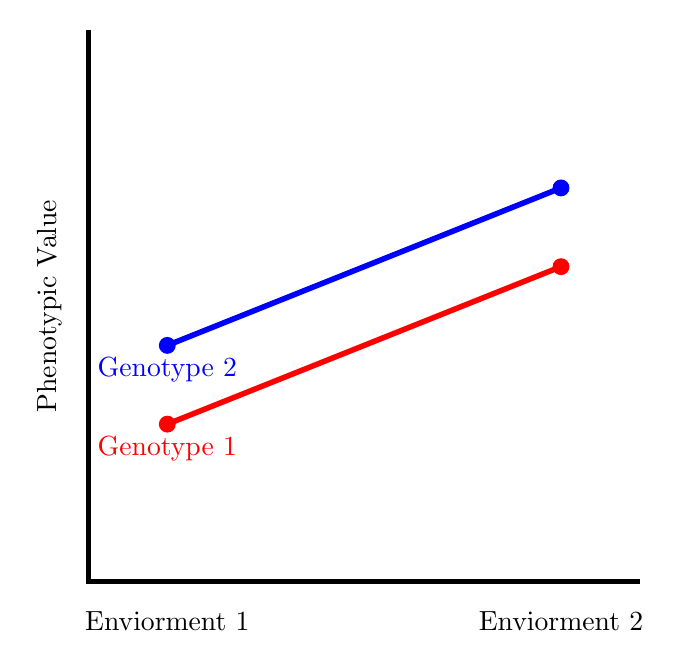
\begin{tikzpicture}
	% axes
	\draw[line width=2, black] (7,0)  -- (0,0) --(0,7);

	% interaction
	\draw[line width=2, red] (1,2) node[below] {Genotype 1}-- (6,4);
	\draw[red, fill=red] (1,2) circle (0.1cm);
	\draw[red, fill=red] (6,4) circle (0.1cm);

	\draw[line width=2, blue] (1,3) node[below] {Genotype 2}-- (6,5);
	\draw[blue, fill=blue] (1,3) circle (0.1cm);
	\draw[blue, fill=blue] (6,5) circle (0.1cm);

	% text
	\node at (1,-0.5) {Enviorment 1};
	\node at (6,-0.5) {Enviorment 2};
	\node[rotate=90] at (-0.5,3.5) {Phenotypic Value};
\end{tikzpicture}

		\caption{Phenotypic Plasticity}
		\label{fig:plasticity}
	\end{subfigure}
	\begin{subfigure}
		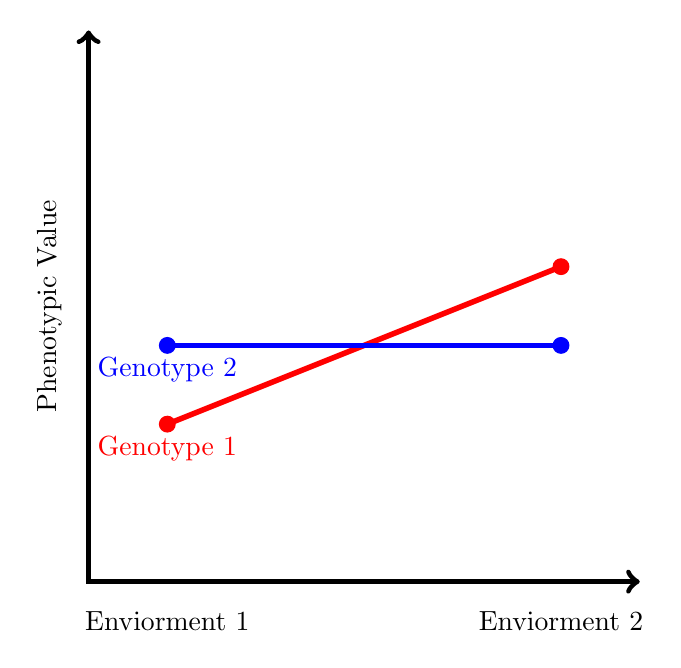
\begin{tikzpicture}
	% axes
	\draw[line width=2, black, <->] (7,0)  -- (0,0) --(0,7);

	% interaction
	\draw[line width=2, red] (1,2) node[below] {Genotype 1}-- (6,4);
	\draw[red, fill=red] (1,2) circle (0.1cm);
	\draw[red, fill=red] (6,4) circle (0.1cm);

	\draw[line width=2, blue] (1,3) node[below] {Genotype 2}-- (6,3);
	\draw[blue, fill=blue] (1,3) circle (0.1cm);
	\draw[blue, fill=blue] (6,3) circle (0.1cm);

	% text
	\node at (1,-0.5) {Enviorment 1};
	\node at (6,-0.5) {Enviorment 2};
	\node[rotate=90] at (-0.5,3.5) {Phenotypic Value};
\end{tikzpicture}

		\caption{Gene-by-Enviorment interaction}
		\label{fig:gene_env_interaction}
	\end{subfigure}
	\label{fig:env_interactions}
	\caption{Different interactions between genes and the enviornment. 
		The colors represent different genotypes. 
		(a) Plasticity. Different enviornments have the same effect on the two genotypes.
		(b) Gene-by-Enviorment Interaction. The effect of the enviornment is genotype specific}
\end{figure}
